% ARPEGOS:  Automatized Roleplaying-game Profile Extensible Generator Ontology based System %
% Author : Alejandro Muñoz Del Álamo %
% Copyright 2019 %

% Section 4.1: Modelo Conceptual %
%Guineforst es un planeta de niebla etérea e islas flotantes. Su industria a lo steampunk-esque ha florecido a lo largo del siglo pasado, combinada con la presencia saturadora de energías mágicas, resultando en aeronaves gigantescas en los cielos púrpura y armas devastadoras y arcanas. Las islas se han dividido en dos facciones: el Imperio de Avelon y la Coalición Helzuran, ambas en guerra por el control de Guineforst, y posiblemente los lugares desconocidos escondidos detrás de las brechas. La gran cantidad de mágia anima a los ciudadanos a producir artefactos basados en la mágia.

\section{Modelo Conceptual} \label{Modelo_conceptual}
\subsection{Introducción}
Un modelo conceptual es una representación clara y precisa de las características estructurales y comportamentales de un sistema 
utilizando un formato predefinido, de acuerdo con Robinson et al. \autocite*{Robinson2016}, es decir, un patrón que permite 
conocer cómo se comporta un sistema concreto y como está dispuesto. \medskip

Uno de los principales objetivos de este proyecto consiste en elaborar un banco de modelos que permita al usuario 
acceder a los juegos cuyo modelo esté incluido, de manera que pueda interactuar con información de diferentes \textit{RPGs} 
sin la necesidad de cambiar de aplicación. Esto resulta sencillo para juegos con mecánicas similares, ya que varía la información
del juego, pero la estructura del proceso de creación se mantiene intacta.\medskip 

El problema surge cuando tratamos de utilizar juegos con mecánicas diferentes, pues el proceso de creación debe 
modificarse parcial o completamente, pero a su vez debe ofrecer toda la información requerida por el usuario para 
proceder a la creación de personajes. Además, no todos los juegos tienen el mismo grado de complejidad, puesto que 
hay juegos que requieren multitud de elementos para la creación de personajes, mientras otros juegos sólo necesitan 
el nombre del personaje y la imaginación del usuario. \medskip

Cada juego tiene su propio \"universo\", en el que se modela un mundo con unas reglas concretas. Para que la aplicación sea 
capaz de procesar todos los universos, representados mediante ontologías, se hace necesario \textit{generalizar} la 
estructura de estas, de manera que el sistema de acceso a la información sea idéntico para todas las ontologías, pero 
cada una de ellas pueda ser explotada de forma completa. \medskip

Así pues, en vez de realizar un modelo conceptual sobre una ontología específica, se va a formular un modelo 
conceptual \textbf{genérico}, que permita identificar los diferentes tipos de elementos de los que puede disponer 
cualquier ontología que vaya a formar parte del banco de datos de la aplicación. \medskip 

Una vez aclarado que el modelo conceptual será genérico, cabe destacar que para realizar una generalización, es necesario 
trabajar con un elemento de pruebas como ejemplo, que permita al equipo de desarrollo abstraer los aspectos generales del 
juego y obtener un modelo eficaz que pueda ser implementado. \medskip 

Durante todo el proyecto, se utilizará como juego de ejemplo \textbf{Ánima: Beyond Fantasy} (al que llamaremos \textit\textbf{{Ánima}} para abreviar). Esto se debe a
que tiene un nivel de complejidad alto en comparación con otros juegos, lo que permite a los desarrolladores considerar que, 
si el modelo es útil para \anima, entonces es igual de válido para juegos de menor complejidad. \medskip

\subsection{UML}
Actualmente hay una gran variedad de lenguajes para describir arquitecturas software, pero no hay consenso para decidir 
qué conjunto de símbolos y sistema de vista debe ser adoptado de manera general. Según indican Kaur y Singh \autocite{Kaur2015},
el \textit{lenguaje de modelado unificado o \textbf{UML}} posibilita a los desarrolladores describir, mostrar y documentar sistemas 
completos, facilitando su colaboración con perspectivas diferentes, gracias a la disposición de una herramienta que les ayuda 
a alcanzar una base común para comunicarse. \medskip

Teniendo en consideración lo anterior, el equipo de desarrollo ha considerado oportuno realizar el modelo conceptual 
utilizando \textit{UML} como base. Para ello, se utilizará el mismo modelo de transformación de elementos \textit{OWL} a 
\textit{UML} que aplica Ortega en su trabajo \textit{Transformación de ontologías OWL a UML para la indexación y recuperación
mediante esquema basado en grafos} \autocite*{Ortega2015}, ya que facilita una conversión clara de los elementos pertenecientes 
a la ontología a \textit{UML} y viceversa, y asímismo, se puede hacer uso de esta para desarrollar un esquema \textit{UML} para 
realizar su conversión a formato \textit{OWL 2}.

\subsection{Elementos}\label{Elementos_modelo_conceptual}
El modelo conceptual desarrollado, que se muestra en la figura \ref{Diagrama_modelo_conceptual}, está basado en los componentes 
que conforman una ontología y sus propiedades:
\begin{itemize}
    \item \textit{\textbf{Individual}}: Citando a Bock, Fokoue, Haase et al. \autocite*{Bock2012}, un individuo es la 
    representación de un objeto real en el dominio.
    \item \textit{\textbf{Class}}: Una clase es un conjunto de individuos que comparten las mismas propiedades y/o 
    comportamientos.
    \item \textit{\textbf{Object Property}}: Una propiedad objeto es una relación que conecta pares de individuos.
    \item \textit{\textbf{Datatype Property}}: Una propiedad de datos asocia un valor con un individuo.
    \item \textit{\textbf{Annotation Property}}: Una propiedad de anotación provee información extra a una ontología, un axioma 
    o un \textit{Identificador de Recursos Internacionalizado (\textbf{IRI})}.
\end{itemize}

\subsection{Relaciones}
Los elementos del modelo conforman una parte importante, pero éste no quedaría completo sin tratar las relaciones que hay entre 
ellos. Para tratarlas vamos a separarlas en función de los elementos que relacionan.
\subsubsection{Individual}
\begin{itemize}
    \item Un individuo puede o no tener una o varias relaciones de datos.
    \item Un individuo puede o no tener una o varias relaciones de objeto con otro u otros individuos.
    \item Un individuo tiene una o varias propiedades de anotación.
\end{itemize}

\subsubsection{Class}
\begin{itemize}
    \item Una clase puede o no estar formada por un conjunto de individuos.
    \item Una clase puede o no estar relacionada con una o varias clases superiores en la jerarquía.
    \item Una clase está relacionada con una definición de clase.
\end{itemize}

\begin{figure}[H]
    \centering
    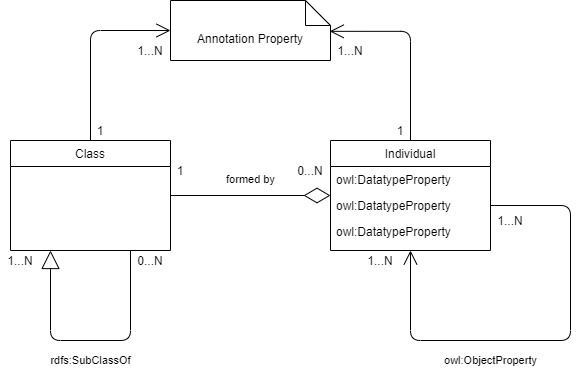
\includegraphics[scale=0.65]{Figures/Modelo_Conceptual.jpg}
    \caption{Modelo conceptual}
    \label{Diagrama_modelo_conceptual}
\end{figure}

